\problemname{Jigsaw Puzzle}

You found a box with old games when cleaning up your attic, and among
them was also a jigsaw puzzle. Unfortunately, the packaging was
damaged, so a couple of puzzle pieces are scattered around the bottom
of the box, and you suspect that some of the pieces may have
been lost elsewhere. In fact, given the orderliness of your attic,
some of the pieces in the box may even come from some entirely
different puzzle! So now you have a pile of puzzle pieces lying in
front of you and you are trying to assemble them into a solved puzzle.

\begin{figure}[!h]
  \centering
  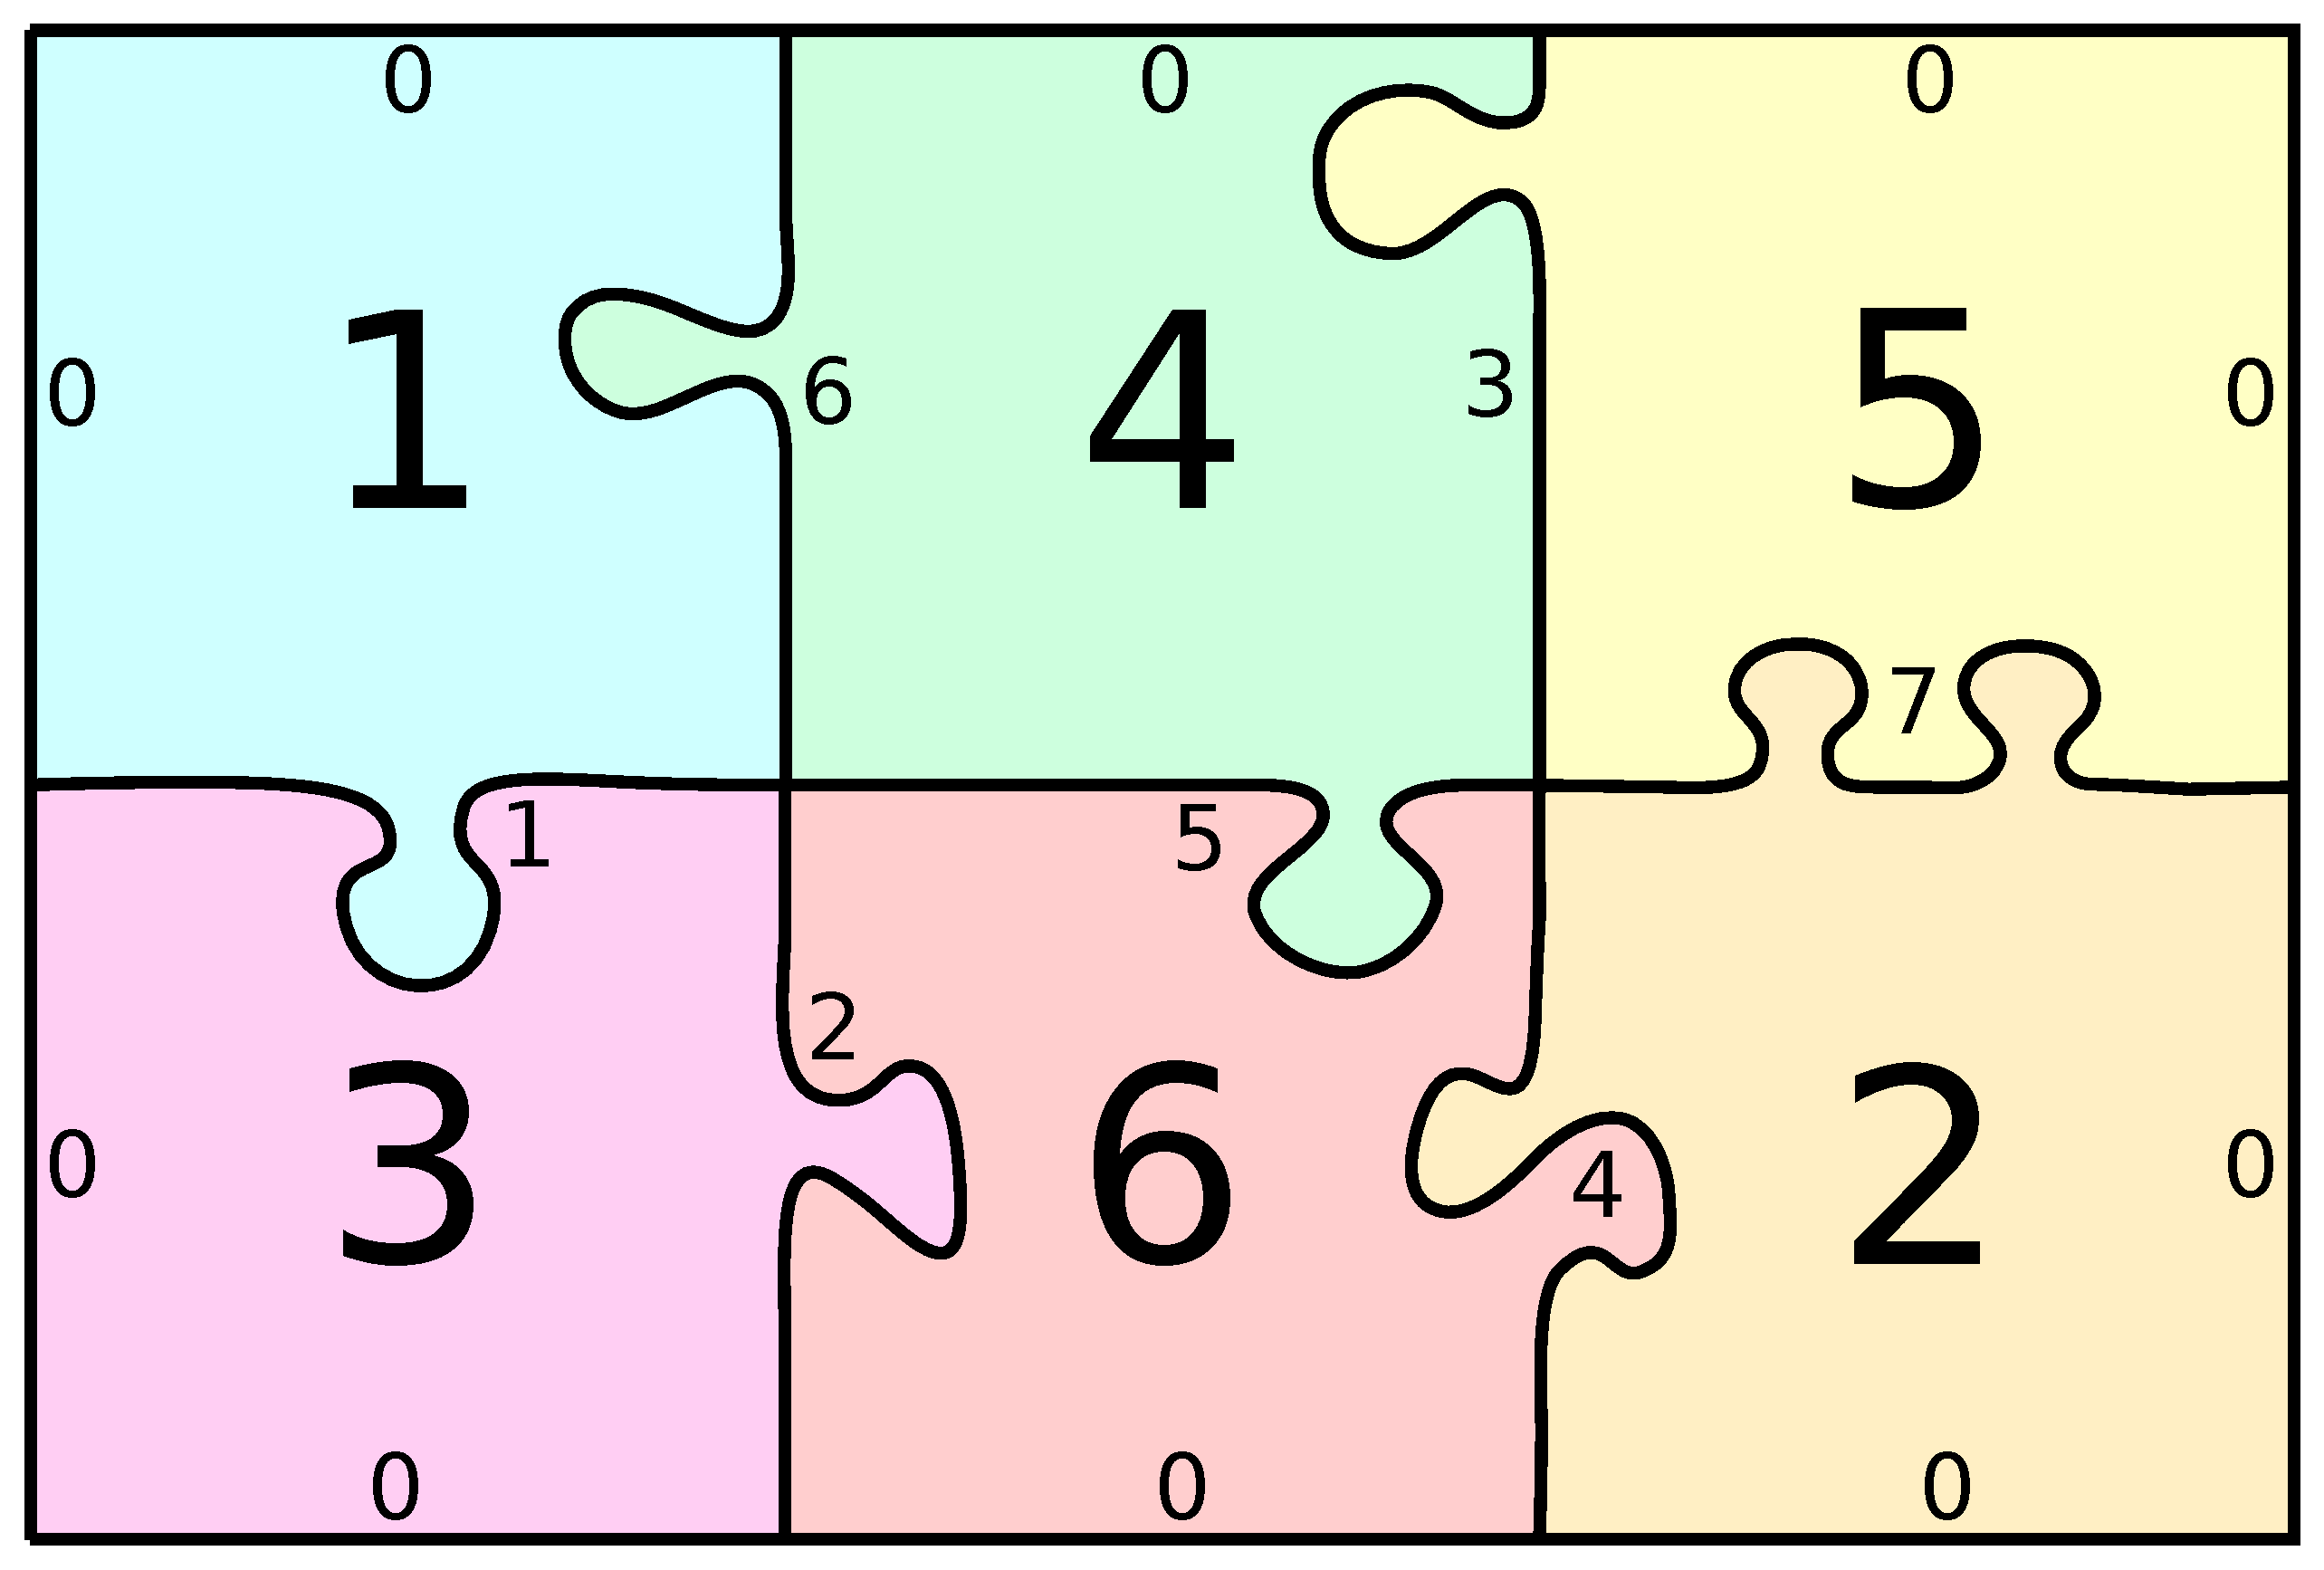
\includegraphics[width=.4\textwidth]{jigsaw.pdf}
  \caption{Illustration of the first sample.}
\end{figure}

More formally:
\begin{itemize}
\item There are $n$ square-shaped pieces, numbered from $1$ to $n$,
  which need to be arranged side by side to form a single rectangle.
  All $n$ pieces have to be used.
\item The edges of the pieces are either straight or irregular.
  Straight edges must be placed on the boundary of the assembled
  rectangle and irregular edges must be placed on the inside.
\item The irregular edges are all shaped differently, so that each
  edge shape occurs exactly two times, on two different puzzle pieces.
  Two pieces can only be placed next to each other if the shapes of
  the corresponding edges match.
\item You may rotate the pieces, but you may not flip them over.
\end{itemize}

\section*{Input}

The input consists of:
\begin{itemize}
  \item one line with one integer $n$ ($1 \le n \le 3 \cdot 10^5$),
    the number of pieces;
  \item $n$ lines, each with four integers, the $i$-th line gives the
    connections (edge shapes) of the $i$-th piece in counter-clockwise
    order.
\end{itemize}

A connection of type $0$ stands for a straight edge.
The other connection types are numbered with consecutive positive
integers starting from $1$ and each of them occurs exactly two times,
on two different lines.

\section*{Output}

If the pieces cannot be assembled as described above, output
\texttt{impossible}. Otherwise, output the solved puzzle in the
following format:
\begin{itemize}
  \item one line with two integers $h,w$ ($h,w \ge 1, h \cdot w = n$),
    the height and width of the grid;
  \item $h$ lines, each with $w$ integers, the numbers of the pieces.
\end{itemize}
Any rotation of the correct solution will by accepted.
